\chapter{The Graph database-based Web Service Composition Approach}\label{C:wd}
This chapter we focuses on the the use of graph databases to model a service repository, with dependencies between the Web services and corresponding compositions being stored in Neo4j graph databases. Our graph based based approach consists of four steps:\par
\begin{enumerate}
  \item Creating graph database for a web service repository: We used all available services in the service repository to create a graph database, with Web services as Nodes and dependencies between services as Edges.\par

  \item Generating a graph database for a given task: We selected all the services related to the given task inputs and outputs, then used related services to generate a graph database.\par

  \item Generating initial population of service composition solutions: We used the graph database we generated in step 2 and the algorithm we designed for this project to produce an initial population of service composition solutions.\par

  \item Selecting a service composition solution from the population with the best overall QoS: We applied the fitness function to the initial population to find the solution with best overall QoS.\par

\end{enumerate}

The overall design of our system is shown as Figure \ref{fig:process}. The following sections will introduce the design in detail.\par
\begin{figure}[h]
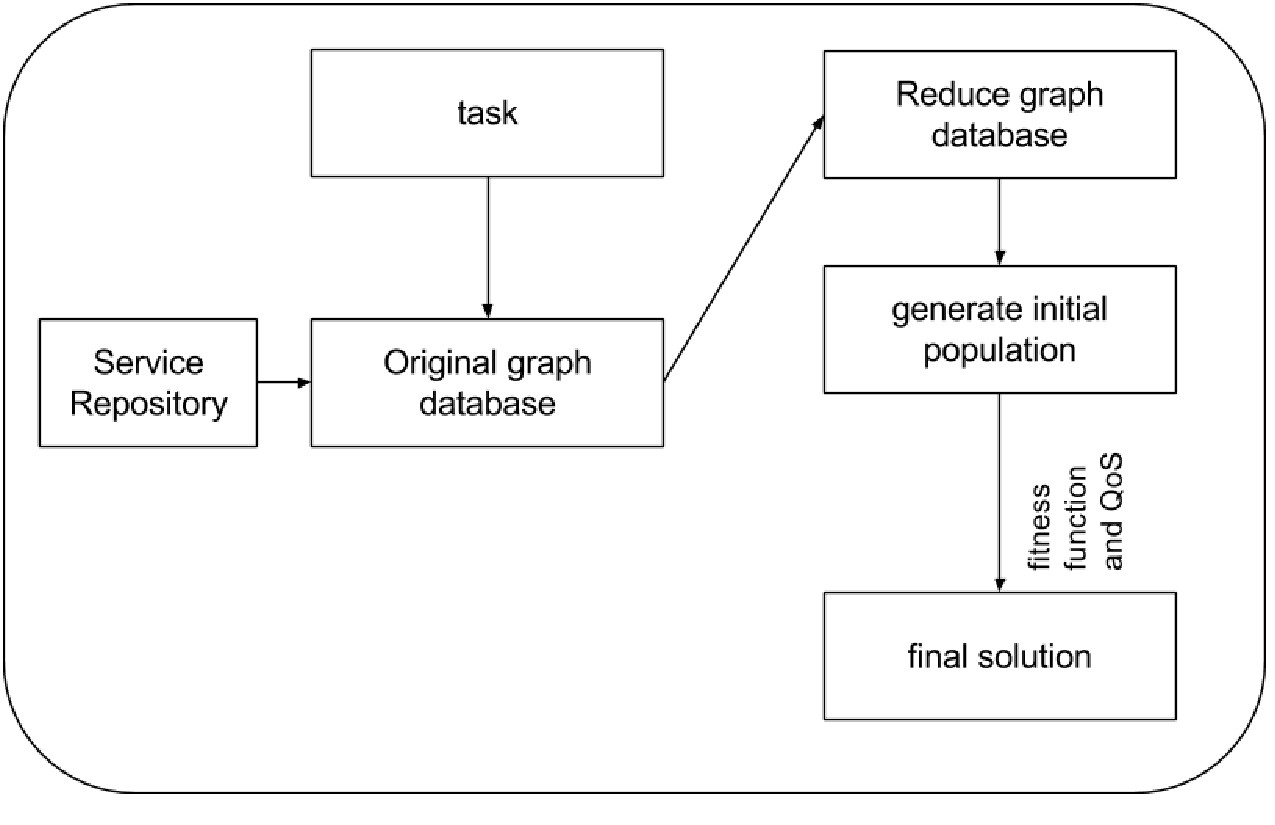
\includegraphics[width=10cm]{process.pdf}
\centering
\caption{Overall system design}
\label{fig:process} 
\end{figure} 

\section{Graph Databases for Web Service Composition} \label{procesedGD}
\subsubsection {Web Service Composition Modeling}
In this project we model a Web service as an entity which has a name, and has a set of properties \emph{name, ID, QoS, inputs, outputs, inputServices, and outputServices}. The first step is to model service repositories, which contains sets of services, that have dependencies between each others. Each service takes inputs, produce outputs, and has QoS. In the following description of our approach we provide details of this model.\par
\subsubsection {Inputs and Outputs}
It is necessary to label each Web service for identification, and the different \emph{inputs} and  \emph{outputs} of each Web service should also be easily identifiable. In our approach we used a taxonomy tree to represent the relationships between the inputs and outputs of services. In the particular taxonomy tree we used, any two concepts \emph{A} and \emph{B} can be related to each other in one of four possible ways. The first scenario is that \emph{A} is a generalization of \emph{B}. The second scenario is that \emph{A} is a specialization of \emph{B}. The third scenario is that \emph{A} and \emph{B} are not related to each other. And the last scenario is that  \emph{A} equals \emph{B}. For example, the Web service \newcommand{\quotes}[1]{``#1''}\quotes{FindHotel} uses a single input parameter (cityName) represented by the concept of \quotes{CITY}, which belongs to the taxonomy tree. Therefore, \quotes{FindHotel} requires an instance of the concept \quotes{CITY}. The only output parameter (Hotel) is represented by an instance of the concept \quotes{Hotel} that also exists in the taxonomy tree. The \emph{inputs} and \emph{outputs} of each Web service are clearly defined in terms of concepts belonging to the specialized taxonomy tree.


\subsubsection {InputServices and OutputServices}
As shown in Figure \ref{fig:inputOutputServs}, within the Neo4j database, Web services are modelled as having a set of \emph{InputServices}, which is the set of Web services connected to the input side of the Web service, and  \emph{outputServices} which is the set of Web services connected to the output side of the service.\par
\begin{figure}[h]
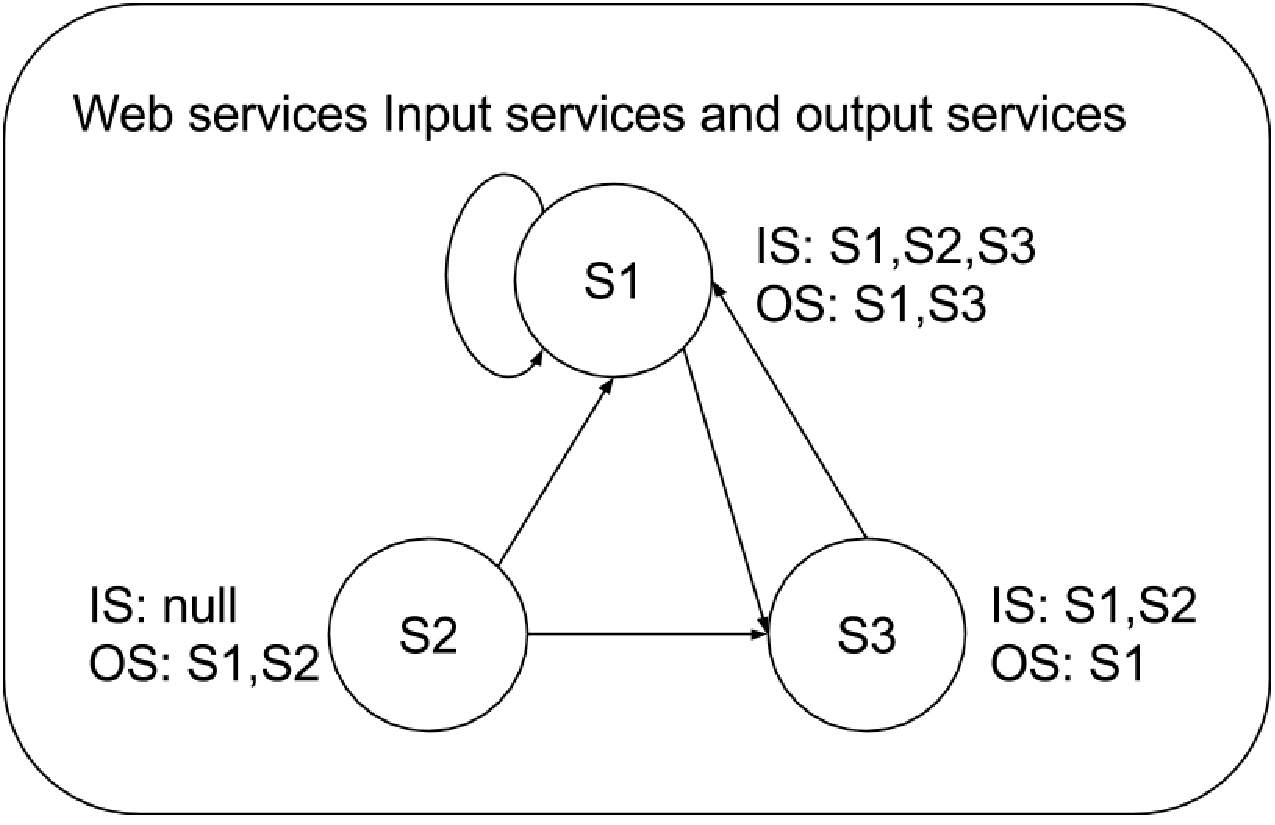
\includegraphics[width=10cm]{InputServicesAndOutServices.pdf}
\centering
\caption{Input services and out services}
\label{fig:inputOutputServs} 
\end{figure} 

\setlength{\textfloatsep}{0pt}% Remove \textfloatsep
\begin{algorithm}[h]
 \SetKwInOut{Input}{Input}\SetKwInOut{Output}{Output}

 \SetKwFunction{connectNode}{connectNode}\SetKwFunction{findCands}{findCands}\SetKwFunction{removeDangling}{removeDangling}
 \LinesNumbered
 \SetNlSty{}{}{:}
  \Input{$taxonomyNodes$, $serviceNodes$}
 \Output{$taxonomyNodes$}
 $i \leftarrow 0$\;
 \While{$i < |taxonomyNodes|$}{\label{buildingLine}
 $tNode \leftarrow taxonomyNodes[i]$\;
 $tNode.parents \leftarrow findParentsNodes(tNode)$\;
 $tNode.children \leftarrow findChildrenNodes(tNode)$\; 
 $i \leftarrow i+1$\;
 }
  $i \leftarrow 0$\;
  \While{$i < | serviceNodes |$}{\label{buildingLine}
       $j \leftarrow 0$\;
       $outputs \leftarrow serviceNodes[i].outputs$\;
      \While{$j < |outputs|$}{\label{buildingLine}
        $tNode \leftarrow findTaxonomyNode(outputs[j])$\;
        $k \leftarrow 0$\;
        \While{$j < |tNode.parents|$}{\label{buildingLine}
          $tNode.parents \leftarrow tNode.parents\cup \{serviceNodes[i]\}$\;
          $k \leftarrow k+1$\;
        }
         $j \leftarrow j+1$\;
      }
       $j \leftarrow 0$\;
       $inputs \leftarrow serviceNodes[i].inputs$\;
       \While{$j < |inputs|$}{\label{buildingLine}
        $tNode \leftarrow findTaxonomyNode(inputs[j])$\;
        $k \leftarrow 0$\;
        \While{$j < |tNode.children|$}{\label{buildingLine}
          $tNode.children \leftarrow tNode.children\cup \{serviceNodes[i]\}$\;
          $k \leftarrow k+1$\;
        }
         $j \leftarrow j+1$\;
      }
 $i \leftarrow i+1$\;
 }
 \caption{\footnotesize Populates the taxonomy tree by associating services with the nodes in the tree.}
\label{generation}
\end{algorithm}
\setlength{\textfloatsep}{20pt}% Remove \textfloatsep
These two properties were added to facilitate the retrieval of connected Web services, and also to reduce the cost of creating relationships between Web services. Algorithm 1, which was designed for this project, identifies all the input and output for each Web service and records them using a taxonomy tree. \par
\begin{figure}[h]
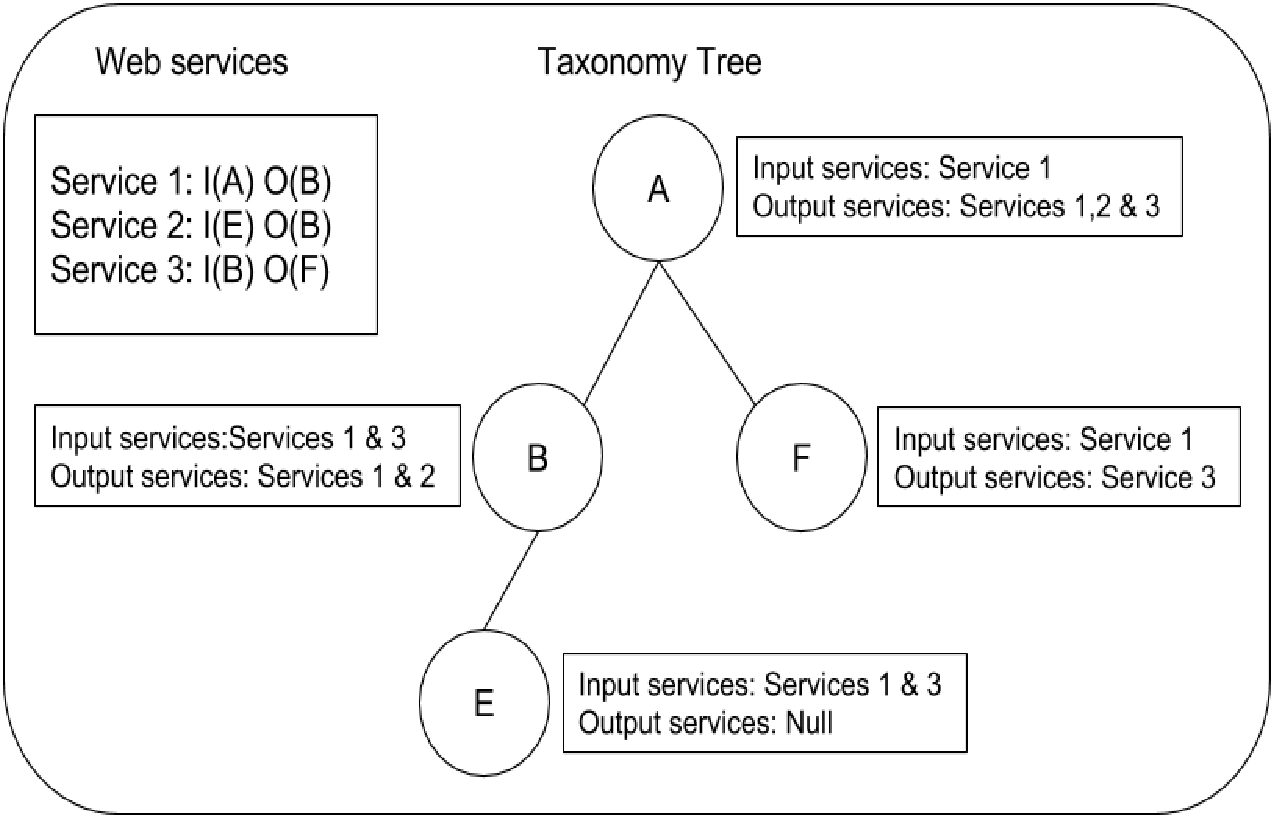
\includegraphics[width = 10cm]{taxonomy-tree-example.pdf}
\centering
\caption{Taxonomy tree Example}
\label{fig:taxonomyTree} 
\end{figure} 
For example, Service \emph{1} has inputs $I_1 = \{A\}$ and outputs $O_1 = \{B\}$, service \emph{2} has Inputs $I_2 = \{E\}$  and outputs $O_2 = \{B\}$, and service \emph{3} has Inputs $I_3 = \{B\}$  and outputs $O_3 = \{F\}$. Algorithm 1 searches services inputs and outputs of services \emph{1, 2} and \emph{3}. Each value in inputs and outputs is a node in the taxonomy tree, which we call a taxonomy node (\emph{tNode}). Each \emph{tNode} has input services (\emph{IS}) and output services (\emph{OS}) fields; then we add Web services into corresponding \emph{IS} or \emph{OS} field. Taxonomy is represented as a tree, and each \emph{tNode} can have a parent node or child node. For example, \quotes{CITY} \emph{tNode} may have parent node called \quotes{COUNTRY} and child node called \quotes{HOTEL}. When we add Web service into \emph{IS}, we also add a Web service into all the \emph{tNode}'s parent node's \emph{IS} field. The same applies to adding Web service into \emph{OS}, in which case we also add Web service into all the \emph{tNode}'s children node's \emph{OS} field. After we run algorithm 1, we obtain $IS_A = \{service 1\}$, $OS_A = \{service 1, service 2, service 3\}$, $IS_B = \{service 1, service 3\}$, $OS_B = \{service 1, service 2\}$, $IS_E = \{service 1, service 3\}$, $OS_E = \{Null\}$, $IS_F = \{service 1\}$ and $OS_F = \{service 3\}$. This is shown in Figure \ref{fig:taxonomyTree}. \par

Algorithm 2 goes through each input value in each Web service (\emph{WS}) in a service repository and finds a corresponding taxonomy node \emph{tNode} and then adds all the input services into the \emph{WS}'s \emph{InputServices} field. It also adds all the input services found in all parent taxonomy nodes into \emph{WS}'s \emph{IS} field. Additionally, it checks each output value in each \emph{WS} in a repository, and finds corresponding \emph{tNode} , adding all the output services into the \emph{WS}'s \emph{OS} field, and all the output services found in all parent taxonomy nodes into \emph{WS}'s \emph{OS} field.

For example,  After we run the algorithm 2, we get: 
Service \emph{1} $IS_1 = \{service 1, service 2, service 3\}$,
Service \emph{1} $OS_1 = \{service 1, service 3\}$,
Service \emph{2} $IS_2 = \{Null\}$,
Service \emph{2} $OS_2 = \{service 1, service 2\}$,
Service \emph{3} $IS_3 = \{service 1, service 2\}$,
Service \emph{3} $OS_3 = \{service 1\}$, shown in Figure \ref{fig:inputOutputServs}.
\begin{algorithm}[h]
 \SetKwInOut{Input}{Input}\SetKwInOut{Output}{Output}
 \SetKwFunction{connectNode}{connectNode}\SetKwFunction{findCands}{findCands}\SetKwFunction{removeDangling}{removeDangling}
 \LinesNumbered
 \SetNlSty{}{}{:}
 \Input{$serviceNodes$}
 \Output{$serviceNodes$}
 $i \leftarrow 0$\;
 \While{$i < |serviceNodes|$}{\label{buildingLine}
   $sNode \leftarrow serviceNodes[i]$\;
   $sNode.inputServices \leftarrow \{\}$\;
   $sNode.outputServices \leftarrow \{\}$\;
   $j \leftarrow 0$\;
     \While{$j < |sNode.outputs|$}{\label{buildingLine}
        $tNode \leftarrow findTaxonomyNode(sNode.outputs[j])$\;
        $k \leftarrow 0$\;
      \While{$k < |tNode.outputServices|$}{\label{buildingLine}

          $sNode.outputServices \leftarrow sNode.outputServices\cup \{tNode.outputServices[k]\}$\;
          $k \leftarrow k+1$\;
      }
        $j \leftarrow j+1$\;
     }
      $j \leftarrow 0$\;
     \While{$j < |sNode.inputs|$}{\label{buildingLine}
        $tNode \leftarrow findTaxonomyNode(sNode.inputs[j])$\;
        $k \leftarrow 0$\;
      \While{$k < |tNode.inputServices|$}{\label{buildingLine}

          $sNode.inputServices \leftarrow sNode.inputServices\cup \{tNode.inputServices[k]\}$\;
          $k \leftarrow k+1$\;
      }
        $j \leftarrow j+1$\;
     }
   $i \leftarrow i+1$\;
 }
 
 \caption{\footnotesize add correspondence input services and output services to each Web service.}
\label{generation}
\end{algorithm}
\setlength{\textfloatsep}{20pt}% Remove \textfloatsep

\subsubsection {Web Service Dependencies}
Each relationship is a directed edge that connects the output of a Web service node to the input of another node according to already established dependencies stored in the taxonomy tree. Like Web service nodes, relationships also have properties. They have a from node, a to node and direction. Relationships between Web service nodes are an essential part of a graph database. They allow us to find related Web services. In our project, we use relationships to solve composition problems. \par
Algorithm 3 handles the process of creating relationships between Web services. It goes through each Web service node \emph{N}, and loops through the corresponding \emph{inputServices} of each \emph{N}, and then adds relationships between the Web services according to the sets of \emph{inputServices}.

\setlength{\textfloatsep}{20pt}% Remove \textfloatsep
\begin{algorithm}[H]
 \SetKwInOut{Input}{Input}\SetKwInOut{Output}{Output}
 \SetKwFunction{connectNode}{connectNode}\SetKwFunction{findCands}{findCands}\SetKwFunction{removeDangling}{removeDangling}
 \LinesNumbered
 \SetNlSty{}{}{:}
 \Input{$serviceNodes$}
 \Output{$serviceNodes$}
 $i \leftarrow 0$\;
 \While{$i < |serviceNodes|$}{\label{buildingLine}
   $sNode \leftarrow serviceNodes[i]$\;
   $j \leftarrow 0$\;
     \While{$j < |sNode.inputServices|$}{\label{buildingLine}
      $inputSNode \leftarrow sNode.inputServices[j]$\;
      $relation \leftarrow inputSNode.createRelationshipTo(sNode)$\;
      $relation.setProperty("From" : inputsNode)$\;
      $relation.setProperty("To" : sNode)$\;
      $relation.setProperty("Outputs" : inputsNode.outputs)$\;
      $relation.setProperty("Direction" : incoming)$\;
        $j \leftarrow j+1$\;
      }
     $i \leftarrow i+1$\;
  }
 \caption{\footnotesize create relationships between Web services.}
\label{generation}
\end{algorithm}
\setlength{\textfloatsep}{20pt}% Remove \textfloatsep

Figure \ref{fig:beforeReduction} is an example of a graph database before reduction. The data set used in this example is WSC 2008 - 01, which contains is a total of 158 Web services. All the nodes represent the Web services and all the edges are the relationships between Web services. Once you click a node or an edge from the graph database, the properties of that node or edge appear at the bottom of the page. Figure \ref{fig:servProp} is an example of the properties that appear when you click the node Web service serv7231183. \par

\begin{figure}[h]
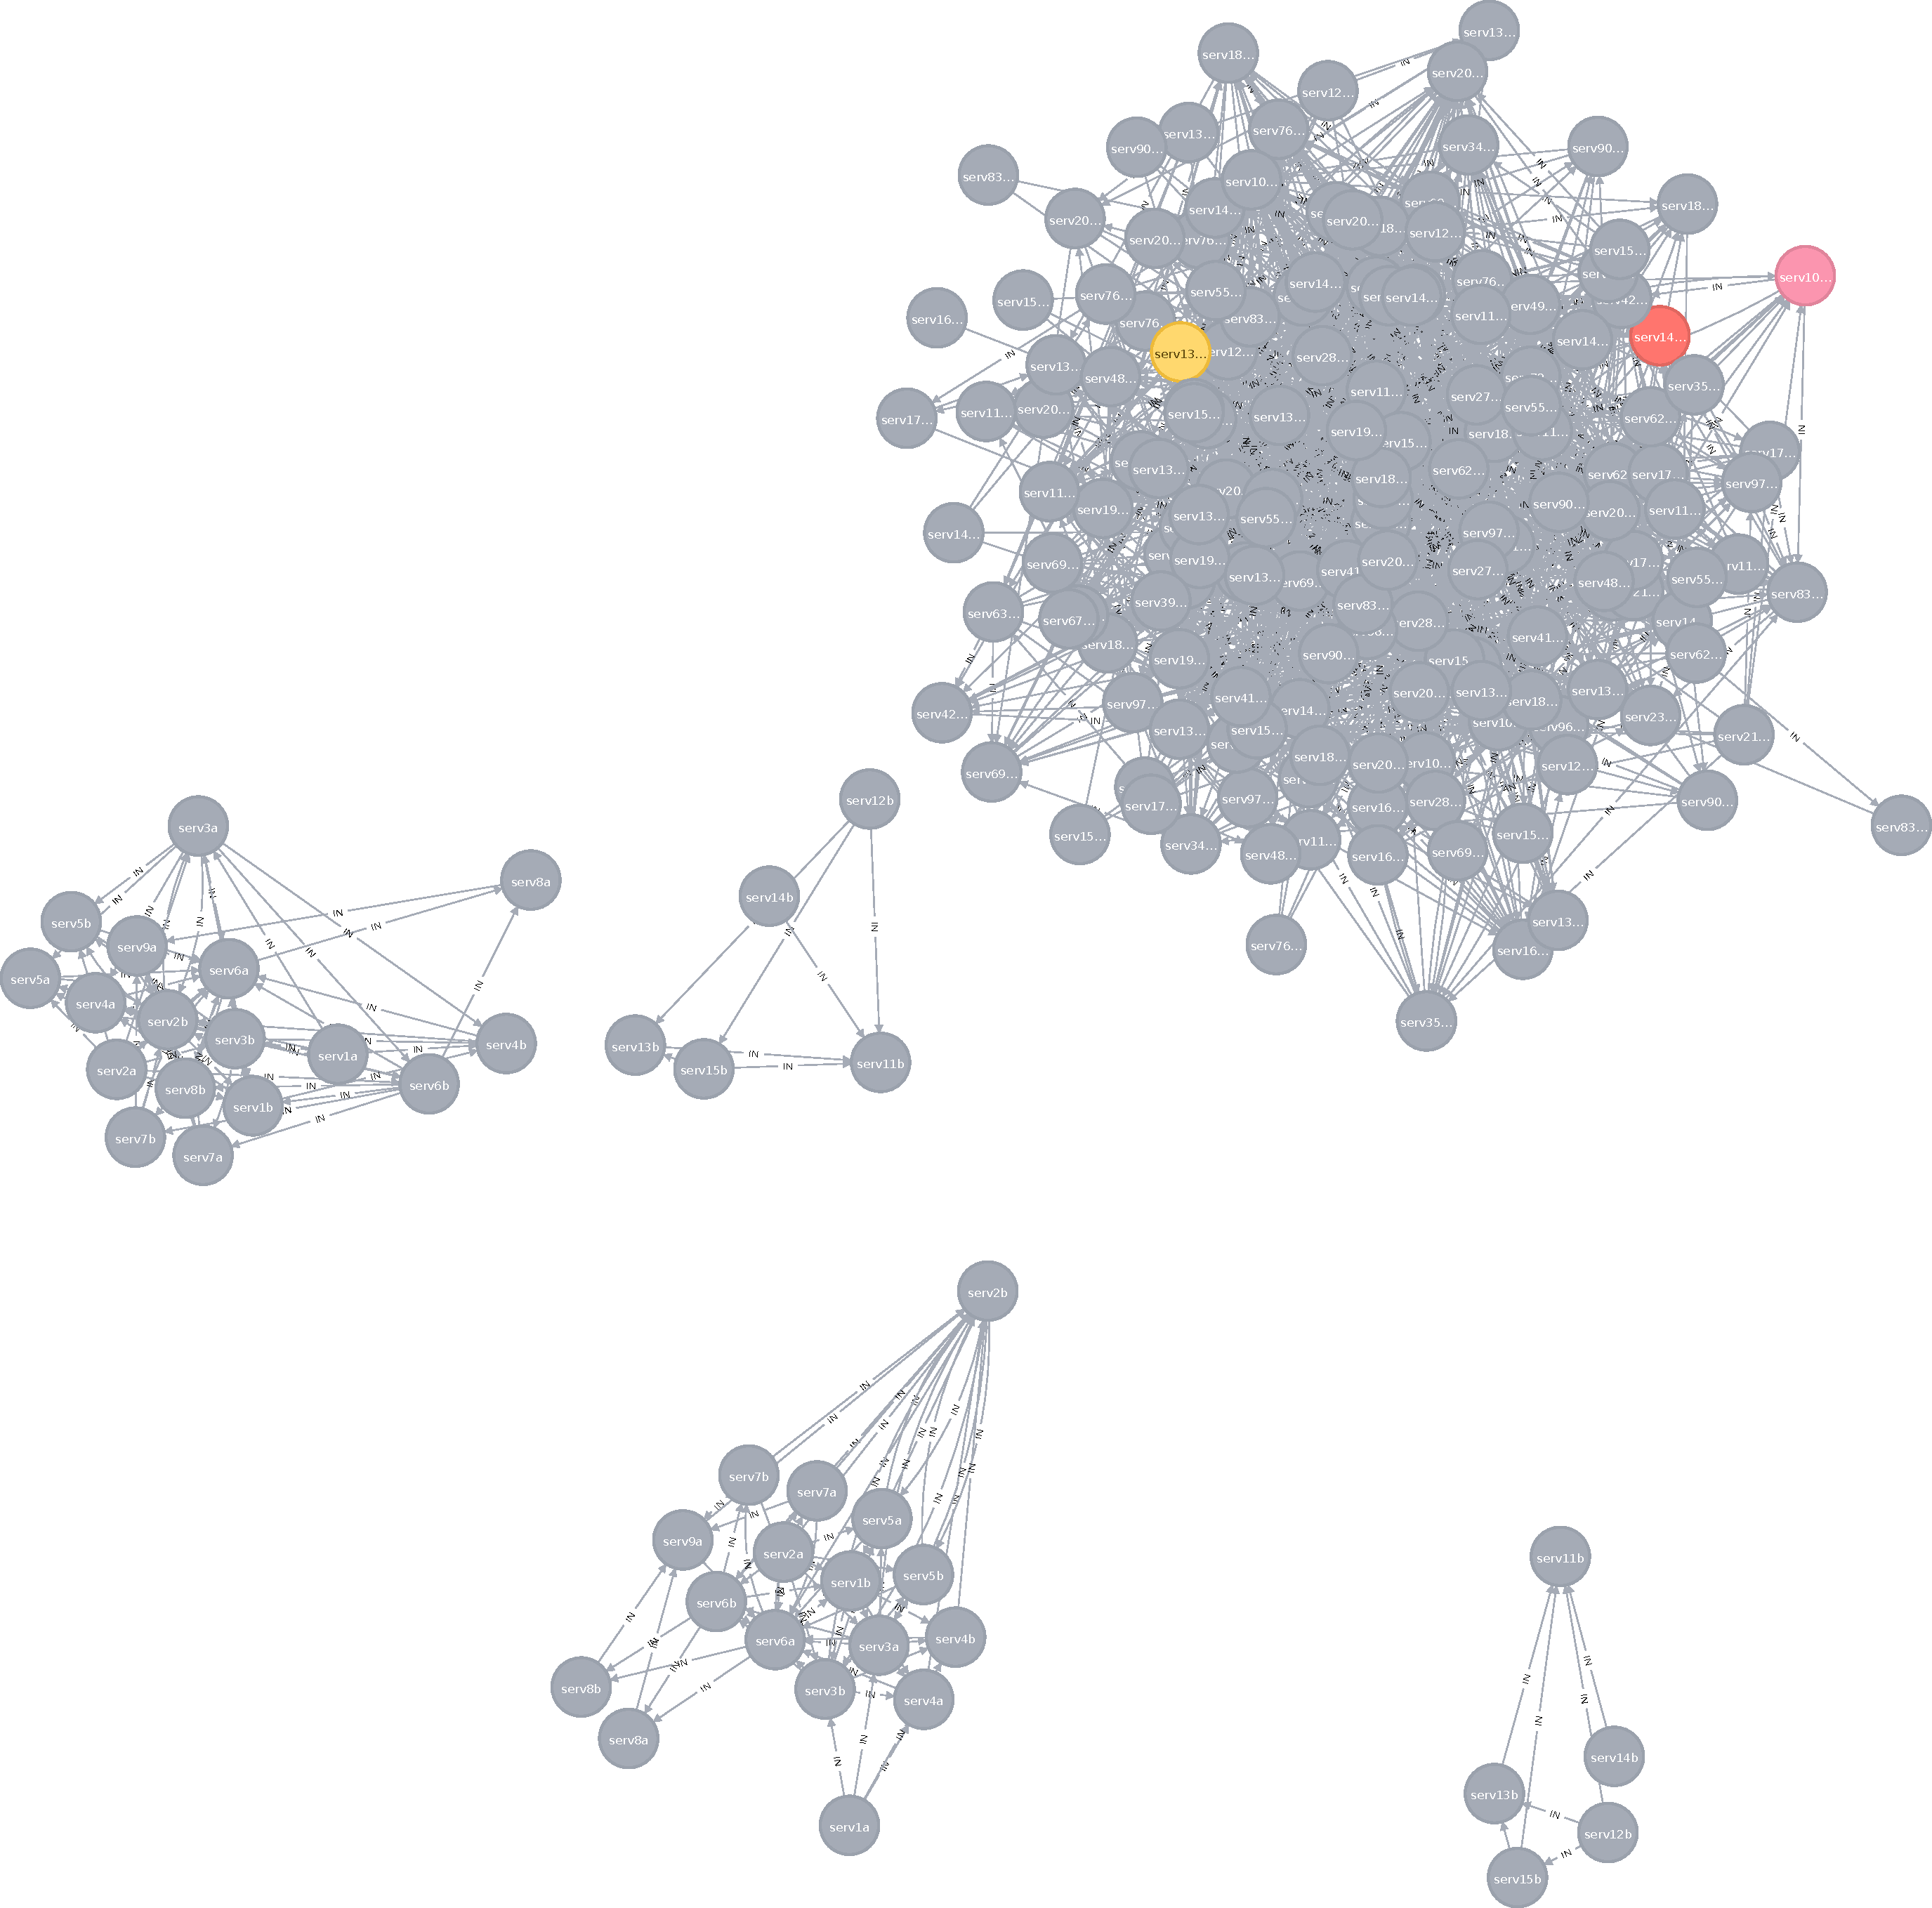
\includegraphics[width = 13cm, height = 10cm, scale = 0.5]{svg-before-reduce.pdf}
\centering
\caption{Graph database before reduction (WSC 2008 - 01)}
\label{fig:beforeReduction} 
\end{figure} 

\begin{figure}[h]
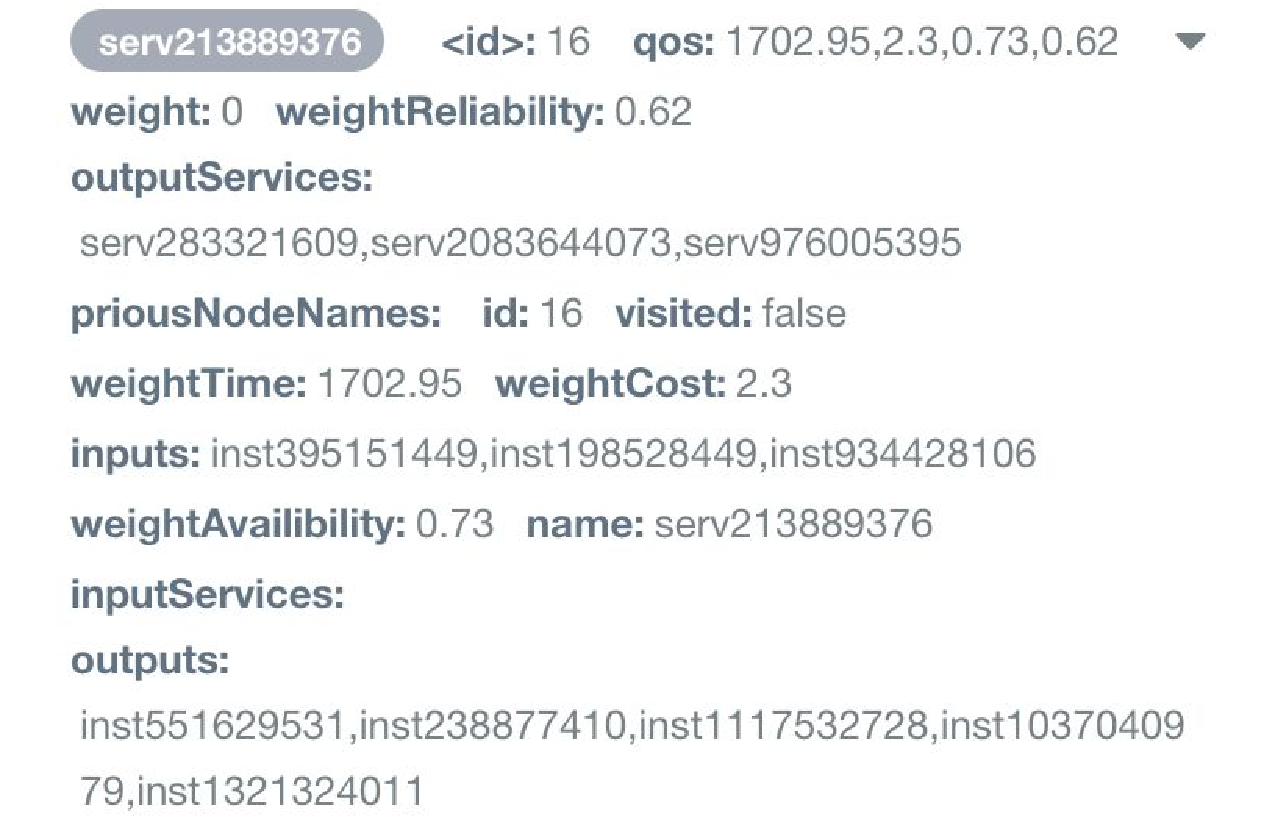
\includegraphics[scale = 0.6]{The-properties-of-Web-service-serv213889376.pdf}
\centering
\caption{The properties of Web service serv7231183 (WSC 2008 - 01)}
\label{fig:servProp} 
\end{figure} 

\section{Graph Databases for a Given Task}
For each given task, only a subset of services in a repository are related to that task. Therefore we created a graph database for each given task. This section presents an algorithm that generates a reduced graph for a given task. \\

\begin{algorithm}[h]
 \SetKwInOut{Input}{Input}\SetKwInOut{Output}{Output}
 \SetKwFunction{connectNode}{connectNode}\SetKwFunction{findCands}{findCands}\SetKwFunction{removeDangling}{removeDangling}
 \LinesNumbered
 \SetNlSty{}{}{:}
  \Input{$serviceNodes$}
 \Output{$relatedNodes$}
 $i \leftarrow 0$\;
 $relatedNodes \leftarrow \{\}$\;
 \While{$i < |serviceNodes|$}{\label{buildingLine}
   $sNode \leftarrow serviceNodes[i]$\;
   \If {$hasRelationship(sNode, startNode) \wedge hasRelationship(sNode, endNode)$}{\label{buildingLine}
        $relatedNodes \leftarrow relatedNodes\cup \{sNode\}$\;
   }
   \If {$!fulfillInputs(sNode)$}{\label{buildingLine}
      $removeRelatedNodes(sNode)$\;
   }
   $i \leftarrow i+1$\;
  }
  \Return { $relatedNodes $\;}
 \caption{\footnotesize reduce graph database.}
\label{generation}
\end{algorithm}
\setlength{\textfloatsep}{20pt}% Remove \textfloatsep

\par

Our algorithm first creates a start node \emph{S} and an end node \emph{E}. The start node \emph{S} contains the inputs of the task and the end node \emph{E}  contains the outputs of the task. Secondly, we insert these nodes into the database by creating new relationships between start node \emph{S} and all the nodes that use \emph{S}'s input. Similarly, we create relationships between end node \emph{E} and all the nodes that can output data to node \emph{E}. Lastly, we find all services that lie on a path between \emph{S} and \emph{E} and remove all services that are not a path. Algorithm 4 shows the process of reducing the original graph database by removing all nodes which do not lie on a path between \emph{S} and \emph{E}.


The following example illustrates the effectiveness of our proposed algorithm. Applying our graph database reduction algorithm (Algorithm 4) to the graph database shown in Figure \ref{fig:inputOutputServs} leads to the new reduced graph database shown in Figure \ref{fig:reduced}. This new reduced graph database contains only Web services which are related to both task \emph{input} and task \emph{output}. Applying this procedure to the database chosen in this example reduces the number of Web services in the graph database from 158 to 61.

\begin{figure}[h]
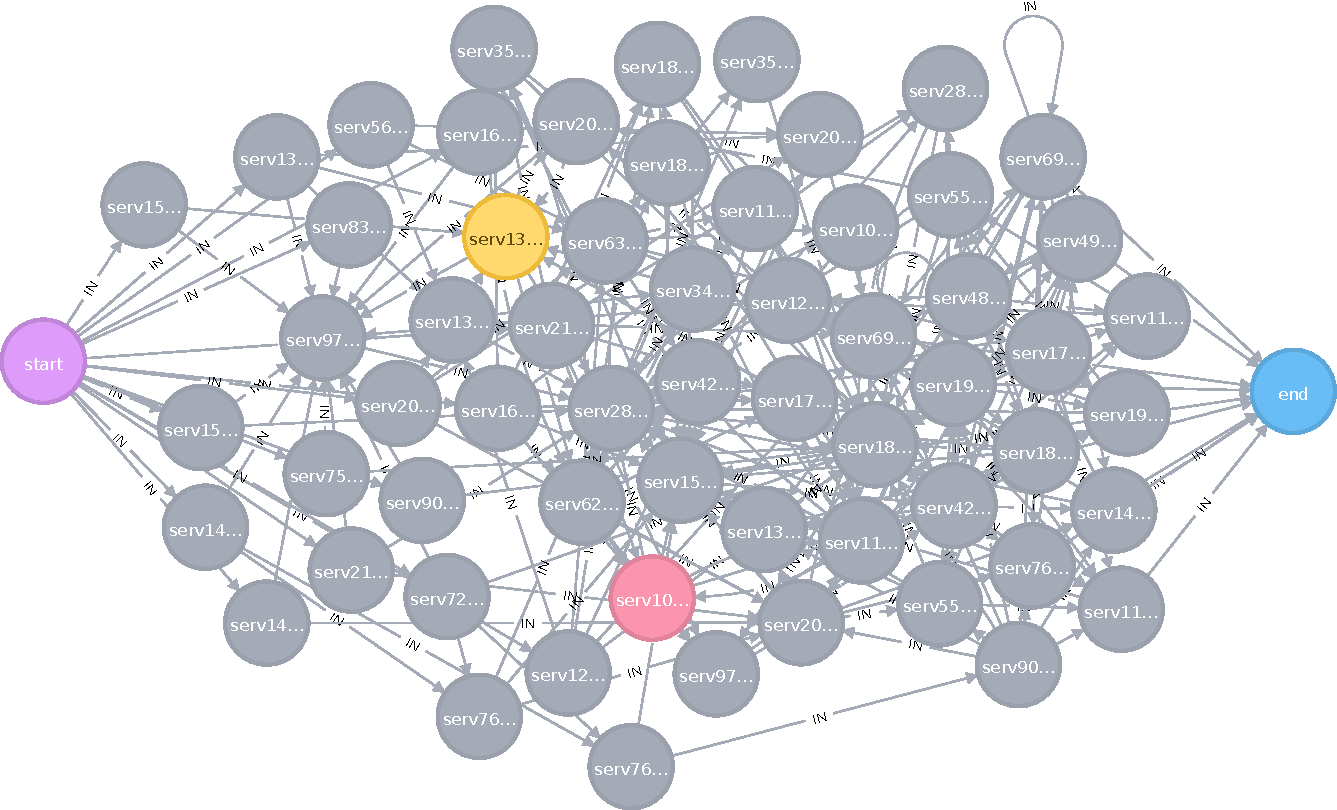
\includegraphics[width = 13cm, height = 10cm, scale = 0.5]{svg-reduced.pdf}
\centering
\caption{Reduced graph database (WSC2008-01)}
\label{fig:reduced} 
\end{figure} 

\section{Generating Web Service Compositions} \label{generatingComp}
Our reduced graph database algorithm allows us to retrieve all the Web service nodes related to a particular task. This section explains how we used related Web service nodes to generate Web service compositions in order to create an initial set of candidates.\par

Algorithm 5 is designed to create feasible compositions. It starts from the end node and searches internal nodes which are directly connected to the end node. Internal nodes are added into the composition list if they fulfill the input of the end node. Then the algorithm recursively goes through each node in the composition list and repeats the above steps until the size of the composition list is stable. This algorithm is also able to calculate the total response time for the creation of each composition,thus determining the total response time from task \emph{input} to task \emph{output}. This total  response time is then used to determine the quality of the solution, when we generate a QoS-Aware service composition. Algorithm 5 calculates the response time during generation of the Web service composition by setting the duration property which reflects the time taken from End Node to Start Node. When adding node \emph{N} to the composition list, the algorithm first checks the \emph{druation} property of node \emph{N}. If \emph{N}'s duration property value is less than the sum of \emph{N}'s previous node  duration property value and  \emph{N}'s execution time ( \emph{N}'s QoS time value), then the algorithm sets  \emph{N}'s duration property value to the sum of the  \emph{N}'s previous node duration property value and  \emph{N}'s execution time.\par

\begin{algorithm}[h]
 \SetKwInOut{Input}{Input}\SetKwInOut{Output}{Output}
 \SetKwFunction{connectNode}{connectNode}\SetKwFunction{findCands}{findCands}\SetKwFunction{removeDangling}{removeDangling}
 \LinesNumbered
 \SetNlSty{}{}{:}
   \Input{$endNode$, $relatedNodes$}
 \Output{Web servie composition}
   $i \leftarrow 0$\;
   $relationships \leftarrow \{\}$\;
   $composition \leftarrow \{\}$\; 
   \While{$i < |getIncomingRelationships(endNode)|$}{\label{buildingLine}
       $relationships \leftarrow relationships\cup \{tNode.getIncomingRelationships(endNode)[i]\}$\;
         $i \leftarrow i+1$\;
   }

   $fulfilledNodes \leftarrow fulfilledNodes \cup \{getNodesFulfillCurrentNode(rels)\}$\;
   \If {$| fulfilledNodes | > 0$}{\label{buildingLine}
        $composition \leftarrow composition\cup \{fulfilledNodes\}$\;
      $j \leftarrow 0$\;
      \While{$i < |composition|$}{\label{buildingLine}
        $Recursively Call This Method Until The Size Of FulfillNodes Equals 0$\;
        $j \leftarrow i+1$\;
      }

   }
 \caption{\footnotesize Web services composition algorithm (initial populations).}
\label{generation}
\end{algorithm}
\setlength{\textfloatsep}{20pt}% Remove \textfloatsep

Two examples of Web service composition are shown in Figure \ref{fig:compEg1} and Figure \ref{fig:compEg2} to illustrate the application of our Web service composition algorithm (Algorithm 5) to the reduced graph database we generated in Figure \ref{fig:reduced}. Both compositions show the relationship between task \emph{input} and task \emph{output}. For each node in the composition it is possible to click the Web service node \emph{S} to find the inputs of \emph{S} and also click the incoming edge of \emph{S} to find the input values related to the Web service which lies at the other end of the edge. \par
\begin{figure}[h]
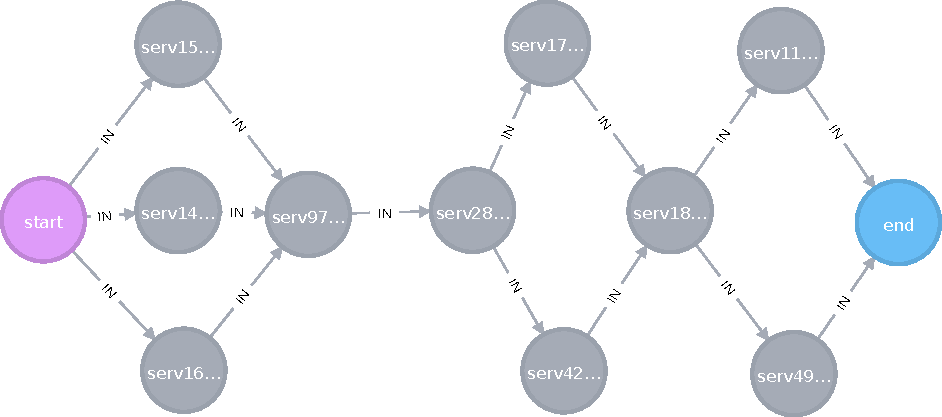
\includegraphics[width=11cm]{svg-composition1.pdf}
\centering
\caption{Web service composition 1 (dataset01, WSC2008)}
\label{fig:compEg1} 
\end{figure} 

\begin{figure}[h]
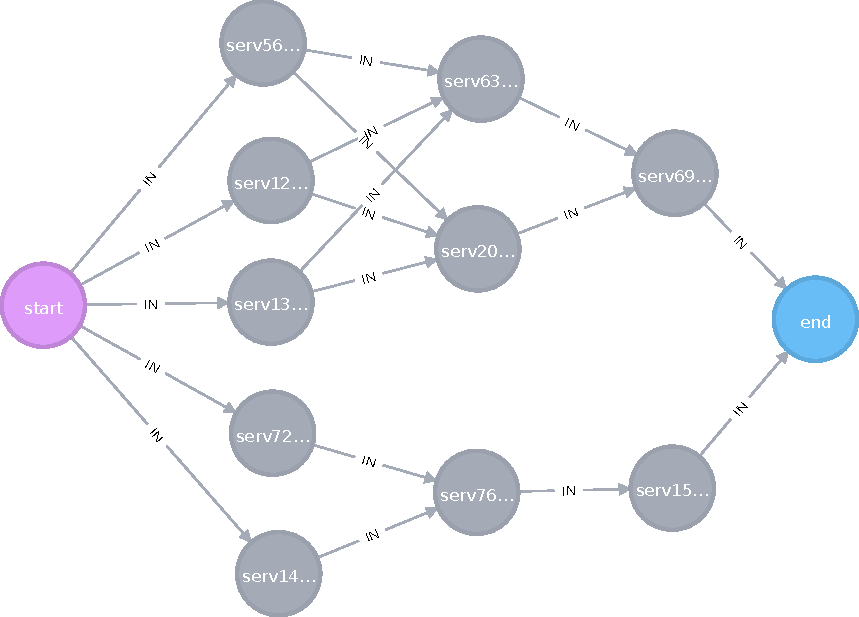
\includegraphics[width=11cm]{svg-composition2.pdf}
\centering
\caption{Web service composition 2 (dataset01, WSC2008)}
\label{fig:compEg2} 
\end{figure} 

\section{QoS-Aware Service Composition}

In section \ref{generatingComp}, we proposed a Web service composition algorithm. The Web service composition algorithm we proposed uses a reduced number of Web services to search for service composition solutions using the smallest number of Web services possible.\par

The next step in our approach is to select a service composition for a set of solutions, which presents the best QoS for a given task. There are many service compositions which can fulfill a given task. As we can see in section 1, to meet a user's non-functional requirements, we must aim to find a service composition that proves to have the best QoS.\par

\begin{algorithm}[h]
 \SetKwInOut{Input}{Input}\SetKwInOut{Output}{Output}

 \SetKwFunction{connectNode}{connectNode}\SetKwFunction{findCands}{findCands}\SetKwFunction{removeDangling}{removeDangling}
 \LinesNumbered
 \SetNlSty{}{}{:}
  \Input{$InitialCompositions$, $weights$}
 \Output{$bestComposition$}
  $i \leftarrow 0$\;
 $BestComposition \leftarrow \{\}$\;
 $BestFintess \leftarrow 0$\; 
 $Map<composition, normalizedList> compWithNormalized \leftarrow \{\}$\;
 \While{$i < |InitialCompositions|$}{\label{buildingLine}
   $j \leftarrow 0$\;
     \While{$j < |InitialCompositions(i)|$}{\label{buildingLine}
      $find (maxC, minC, maxT, minT, maxA, minA, maxR, minR)$\;
      $j \leftarrow j+1$\;
  }
   $i \leftarrow i+1$\;
  }
  $i \leftarrow 0$\;
 \While{$i < |InitialCompositions|$}{\label{buildingLine}
   $j \leftarrow 0$\;
     \While{$j < |InitialCompositions(i)|$}{\label{buildingLine}
        $NormalizedList.add(normalize(Cost, Time, Availability, Availability));$
      $j \leftarrow j+1$\;
     }
     $compWithNormalized.getKey(composition) \leftarrow  NormalizedList;$

   $i \leftarrow i+1$\;
  }

  $i \leftarrow 0$\;
 \While{$i < |compWithNormalized|$}{\label{buildingLine}
    $fitnessValue = fitnessFunction(compWithNormalized(i), weights)$\;
      \If{$fitnessValue > BestFitness$}{
        $BestFitness \leftarrow  fitnessValue$\;
        $BestComposition \leftarrow  composition;$
        }
}
 \caption{\footnotesize QoS aware Web services composition algorithm}
\label{generation}
\end{algorithm}
\setlength{\textfloatsep}{20pt}% Remove \textfloatsep

Algorithm 6 is designed to search for the solution with best QoS. Using the set of initial population generated from Algorithm 5, the algorithm goes through each and every service node invoked in the compositions. It then determines minimums and maximums of execution cost, response time, availability and reliability. Having found all minimums and maximums the next steps are to carry out normalization to restrict all values to the interval \emph{[0,1]}, and then to apply a fitness function, using normalized QoS properties and user defined weights (see section \ref{fitnessFunction}), to each service composition. Lastly, the algorithm returns the service composition which has the best fitness value. \par

The following example shows a comparison of two compositions and uses data from Table \ref{tb:compExample}, which contains QoS properties and fitness values of web service compositions. \\

EXAMPLE SHOWING THE COMPARISON OF TWO WEB SERVICE COMPOSITIONS \\

Composition 1 is shown in Figure \ref{fig:compEg1} and composition  2 is shown in Figure \ref{fig:compEg2}. To determine which is the better of the two compositions, we normalized the QoS properties and used the fitness functions (section \ref{fitnessFunction}) of each service composition. Since we are only using two compositions in this example, the highest values on Availability and reliability, and the lowest values on Cost and Time will be equal or close to 1. We then set the weight for our fitness function to \emph{0.25}. The result in Table \ref{tb:compExample} shows that composition 2 (originally shown in \ref{fig:compEg2}) has the best fitness.  \par


% Please add the following required packages to your document preamble:
% \usepackage{multirow}
\begin{table}[h]
\centering
\caption{Comparison of two web service compositions}
\label{tb:compExample}
\scalebox{0.9}{
\begin{tabular}{|c|c|c|c|c|c|c|}
\hline
\multicolumn{2}{|c|}{\textbf{Compositions}}               & Cost   & Time     & Availability & Reliability & Fitness                 \\ \hline
\multirow{2}{*}{\textbf{1 (Figure \ref{fig:compEg1})}} & Non-normalized & 48.11  & 23427.83 & 1.60043E-5   & 0.00935     & \multirow{2}{*}{0.25}   \\ \cline{2-6}
                                         & Normalized     & 0.0    & 0.0      & 0.0          & 1.0         &                         \\ \hline
\multirow{2}{*}{\textbf{2 (Figure \ref{fig:compEg2})}} & Non-normalized & 44.18  & 12858.46 & 0.005        & 0.001408    & \multirow{2}{*}{0.7475} \\ \cline{2-6}
                                         & Normalized     & 0.9899 & 1.0      & 1.0          & 0.0         &                         \\ \hline
\end{tabular}
}
\end{table}